\documentclass{article}
\usepackage{tikz}

\begin{document}

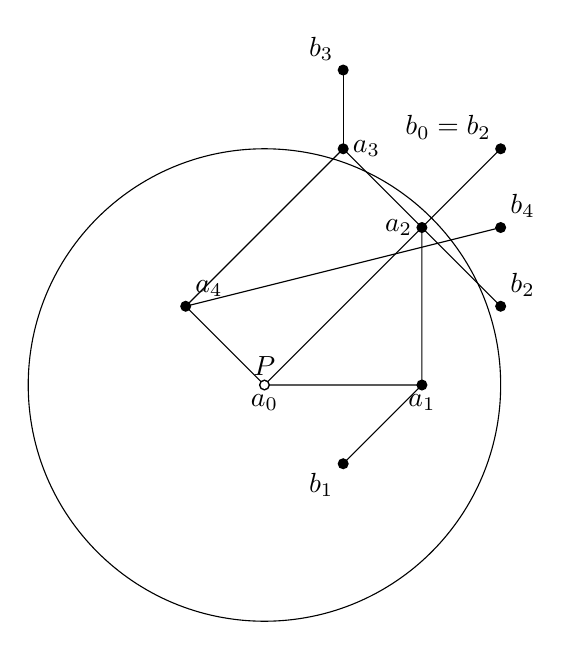
\begin{tikzpicture}[scale=2]
    % Define coordinates
    \coordinate (a0) at (0, 0);
    \coordinate (a1) at (1, 0);
    \coordinate (a2) at (1, 1);
    \coordinate (a3) at (0.5, 1.5);
    \coordinate (a4) at (-0.5, 0.5);
    
    \coordinate (b0) at (1.5, 1.5);
    \coordinate (b1) at (0.5, -0.5);
    \coordinate (b2) at (1.5, 0.5);
    \coordinate (b3) at (0.5, 2);
    \coordinate (b4) at (1.5, 1);
    
    % Draw the polygon P
    \draw (a0) -- (a1) -- (a2) -- (a3) -- (a4) -- cycle;
    
    % Draw the circle
    \draw (0, 0) circle (1.5);
    
    % Draw the lines connecting points on the circle
    \draw (a0) -- (b0);
    \draw (a1) -- (b1);
    \draw (a2) -- (b2);
    \draw (a3) -- (b3);
    \draw (a4) -- (b4);
    
    % Label the points
    \fill (a0) circle (1pt) node[below] {$a_0$};
    \fill (a1) circle (1pt) node[below] {$a_1$};
    \fill (a2) circle (1pt) node[left] {$a_2$};
    \fill (a3) circle (1pt) node[right] {$a_3$};
    \fill (a4) circle (1pt) node[above right] {$a_4$};
    
    \fill (b0) circle (1pt) node[above left] {$b_0 = b_2$};
    \fill (b1) circle (1pt) node[below left] {$b_1$};
    \fill (b2) circle (1pt) node[above right] {$b_2$};
    \fill (b3) circle (1pt) node[above left] {$b_3$};
    \fill (b4) circle (1pt) node[above right] {$b_4$};
    
    % Label the region P
    \node at (0, 0) [circle, fill=white, inner sep=1pt] {};
    \node at (0, 0) [above] {$P$};
\end{tikzpicture}

\end{document}